% !TEX TS-program = xelatex
% !TEX encoding = UTF-8 Unicode
\documentclass[aspectratio=169]{xmu-slide}
\usepackage{amssymb}
\pgfplotsset{compat=1.18}
\usetikzlibrary{shapes.geometric,arrows.meta,positioning,calc}

\title{向量数据库高效检索关键技术研究}
\author{林正刚}
\teacher{沈志荣教授}
\pubdate{2026 年 5 月 18 日}

\begin{document}

\maketitle

\begin{frame}[t]{研究背景与问题动机}
    \small
    \begin{itemize}
        \item 向量数据库支撑推荐、图文检索和 RAG 等应用，查询通常同时包含相似度要求和业务属性约束。
        \item 过滤近似近邻检索要求结果既相似，又满足标签、权限、时间范围等过滤条件。
        \item 过滤条件改变每次查询的有效候选规模，从而影响查询性能。
    \end{itemize}
    \vfill
    \centering
\end{frame}

\begin{frame}[t]{问题定义}
    \small
    \begin{itemize}
        \item 数据集：$D=\{(\bm{x}_i,\lambda_i)\}_{i=1}^N$，其中 $\bm{x}_i$ 为向量，$\lambda_i$ 为标签集合。
        \item 查询：$Q=(q,F,k)$，其中 $q$ 为查询向量，$F$ 为过滤条件，$k$ 为返回结果数。
        \item 有效候选集：$S_F=\{\bm{x}_i\in D\mid P_F(\lambda_i)=1\}$。
        \item {\color{red}选择性}：$\rho(F)=|S_F|/N$，表示过滤后仍可参与检索的数据比例。
        \item 目标：在内存受限场景下，以较低时延返回满足过滤条件且具有高召回率的 top-$k$ 结果。
    \end{itemize}
\end{frame}

\begin{frame}[t]{过滤方法概览}
    \scriptsize
    从系统实现角度，filtered ANN 方法大致可分为两类：在现有 ANN 索引上增强过滤能力，或在建索引阶段显式编码过滤信息。\\[0.35em]
    \centering
    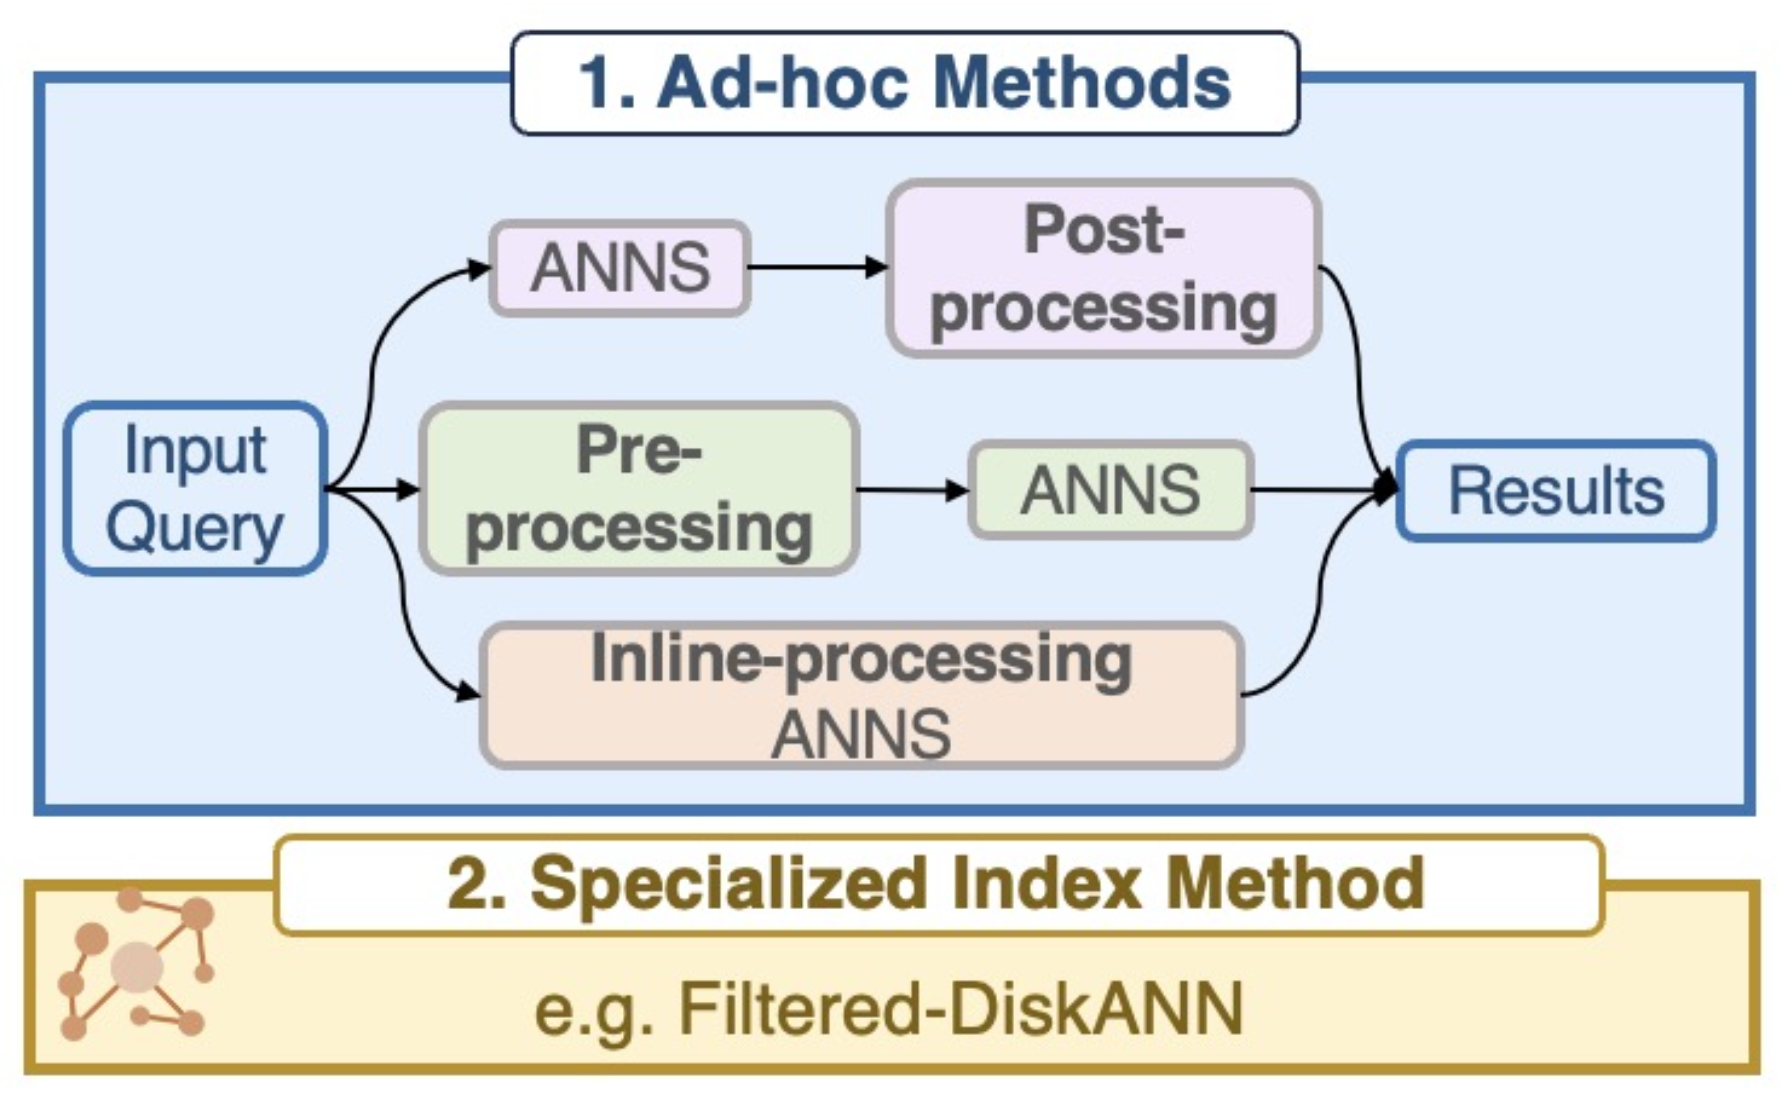
\includegraphics[width=0.96\textwidth,height=0.69\textheight,keepaspectratio]{figures/image.png}
\end{frame}

\begin{frame}[t]{当前挑战}
    \small
    \begin{itemize}
        \item 同一套查询流程，很难同时适配低选择性和高选择性。
        \item \textbf{先过滤后搜索}：低选择性下候选少、开销低；选择性升高后容易退化为对完整数据集的全量扫描与计算。
        \item \textbf{先搜索后过滤与内联处理}：高选择性下由于存在预构建索引，因此有性能优势；但低选择性下会访问大量不符合过滤条件的节点，导致性能急剧恶化。
        \item \textbf{内存受限场景}：先搜索后过滤与内联搜索需要发起 SSD IO 以访问索引，其中对不满足过滤条件的节点发起的 IO 会进一步导致性能退化。
        \item \textbf{过滤感知特殊索引}：类似 Filtered-DiskANN 的方法不支持索引更新；同时由于为所有标签构建子图，会占用大量 SSD 空间。
    \end{itemize}
\end{frame}

\begin{frame}[t]{现有工作与本文贡献}
    \small
    \begin{itemize}
        \setlength{\itemsep}{0.2em}
        \item \textbf{过滤感知图索引}：Filtered-DiskANN [1] 代表面向内存受限场景的过滤图路线，但存在更新能力和空间开销方面的限制。
        \item \textbf{通用内联过滤}：ACORN [2]、UNG [3] 更强调在统一结构中处理不同过滤谓词，减少对特定标签的依赖。
        \item \textbf{向量数据库}：Milvus [4]、Qdrant [5] 等系统支持在传统 DiskANN/HNSW 索引上进行过滤。
        \item \textbf{本文贡献}：在统一索引上使用两个不同的搜索算法，根据不同选择性自动选择最合适的算法。
    \end{itemize}
    \vspace*{\fill}
    \fontsize{3.8}{4.2}\selectfont
    [1] Gollapudi et al. 2023. Filtered-DiskANN: Graph Algorithms for Approximate Nearest Neighbor Search with Filters. \textit{WWW '23}.\\[0.25em]
    [2] Patel et al. 2024. ACORN: Performant and Predicate-Agnostic Search Over Vector Embeddings and Structured Data. \textit{Proc. ACM Manag. Data}.\\[0.25em]
    [3] Cai et al. 2025. Navigating Labels and Vectors: A Unified Approach to Filtered Approximate Nearest Neighbor Search. \textit{Proc. ACM Manag. Data}.\\[0.25em]
    [4] Wang et al. 2021. Milvus: A Purpose-Built Vector Data Management System. \textit{SIGMOD '21}.\\[0.25em]
    [5] Qdrant Team. 2023. Qdrant: High-performance vector search engine.
\end{frame}

\begin{frame}[t]{系统架构}
    \begin{columns}[T]
        \column{0.56\textwidth}
        \vspace{-0.25em}
        \small
        \begin{itemize}
            \setlength{\itemsep}{0.15em}
            \item 查询进入系统后，先根据过滤条件估计选择性 $\rho(F)$。
            \item 框架保留两条互补路径：
                {\setbeamerfont{itemize/enumerate subbody}{size=\small}
                \setbeamerfont{enumerate subitem}{size=\small}
                \setbeamerfont{subitem projected}{size=\small}
                \setlength{\itemsep}{0.06em}
                  \begin{enumerate}
                      \item \textbf{先过滤后搜索}：生成候选集，PQ 排序，再读取少量原始向量重排序。
                      \item \textbf{内联过滤}：沿用 PipeANN$^{[1]}$ 图搜索，在节点访问过程中判断过滤条件。
                  \end{enumerate}
                  }
            \item 低选择性走左侧路径，高选择性走右侧路径；两条路径共享索引、PQ 编码和标签接口。
        \end{itemize}
        \vspace{-0.05em}
        \fontsize{4.1}{4.5}\selectfont
        [1] Hao Guo and Youyou Lu. 2026. Achieving Low-Latency Graph-Based Vector Search via Aligning Best-First Search Algorithm with SSD. \textit{ACM Trans. Storage} 22, 2, Article 12.

        \column{0.44\textwidth}
        \centering
        \resizebox{0.91\textwidth}{!}{%
        \begin{tikzpicture}[
            node distance=0.36cm,
            box/.style={rectangle, draw, rounded corners=2pt, text width=2.45cm, align=center,
                        minimum height=0.56cm, font=\fontsize{5.6}{6.2}\selectfont, inner sep=2.8pt},
            dec/.style={diamond, draw, aspect=3.3, text width=2.65cm, align=center,
                        font=\fontsize{5.6}{6.2}\selectfont, inner sep=2.2pt},
            >=Stealth, thick
        ]
        \node[box] (input) {查询 $(q,\,F,\,k)$};
        \node[box, below=of input] (sel) {读取标签预计算选择性 $\rho(F)$};
        \node[dec, below=0.5cm of sel] (route) {$\rho(F) < \tau$ ?};

        \node[box] (bitset) at ($(route)+(-2.35cm,-1.75cm)$)
            {位图生成候选集 $S_F$};
        \node[box, below=of bitset] (pq)    {PQ 近似距离计算};
        \node[box, below=of pq]    (topLr)  {选取 PQ 距离最近\\的少量候选};
        \node[box, below=of topLr] (ssd1)   {从 SSD 读取原始向量\\计算精确距离};

        \node[box] (graph) at ($(route)+(2.35cm,-1.75cm)$)
            {PipeANN$^{[1]}$ 图搜索};
        \node[box, below=of graph] (filter) {节点展开时执行过滤判断};

        \coordinate (outy) at ($(ssd1.south)+(0,-0.55cm)$);
        \node[box] (output) at (outy -| sel) {返回满足条件的 top-$k$ 结果};

        \draw[->] (input) -- (sel);
        \draw[->] (sel) -- (route);

        \path (route.west) -- (bitset.north |- route.west) coordinate[midway] (lmid);
        \path (route.east) -- (graph.north |- route.east) coordinate[midway] (rmid);
        \draw[->] (route.west) -| (bitset.north);
        \draw[->] (route.east) -| (graph.north);
        \node[font=\fontsize{4.8}{5.2}\selectfont, above=1pt] at (lmid) {是};
        \node[font=\fontsize{4.8}{5.2}\selectfont, above=1pt] at (rmid) {否};

        \draw[->] (bitset) -- (pq);
        \draw[->] (pq) -- (topLr);
        \draw[->] (topLr) -- (ssd1);
        \draw[->] (ssd1.south) |- (output.west);

        \draw[->] (graph) -- (filter);
        \draw[->] (filter.south) |- (output.east);
        \end{tikzpicture}%
        }
    \end{columns}
\end{frame}

\begin{frame}[t]{设计点 1：混合搜索架构}
    \scriptsize
    \textbf{核心观察：}两条路径的优势区间不同，延迟曲线会随选择性发生交叉。\\[0.35em]
    \textbf{设计选择：}低选择性使用先过滤后搜索，高选择性回到 PipeANN 图搜索中的内联过滤。\\[0.45em]
    \centering
    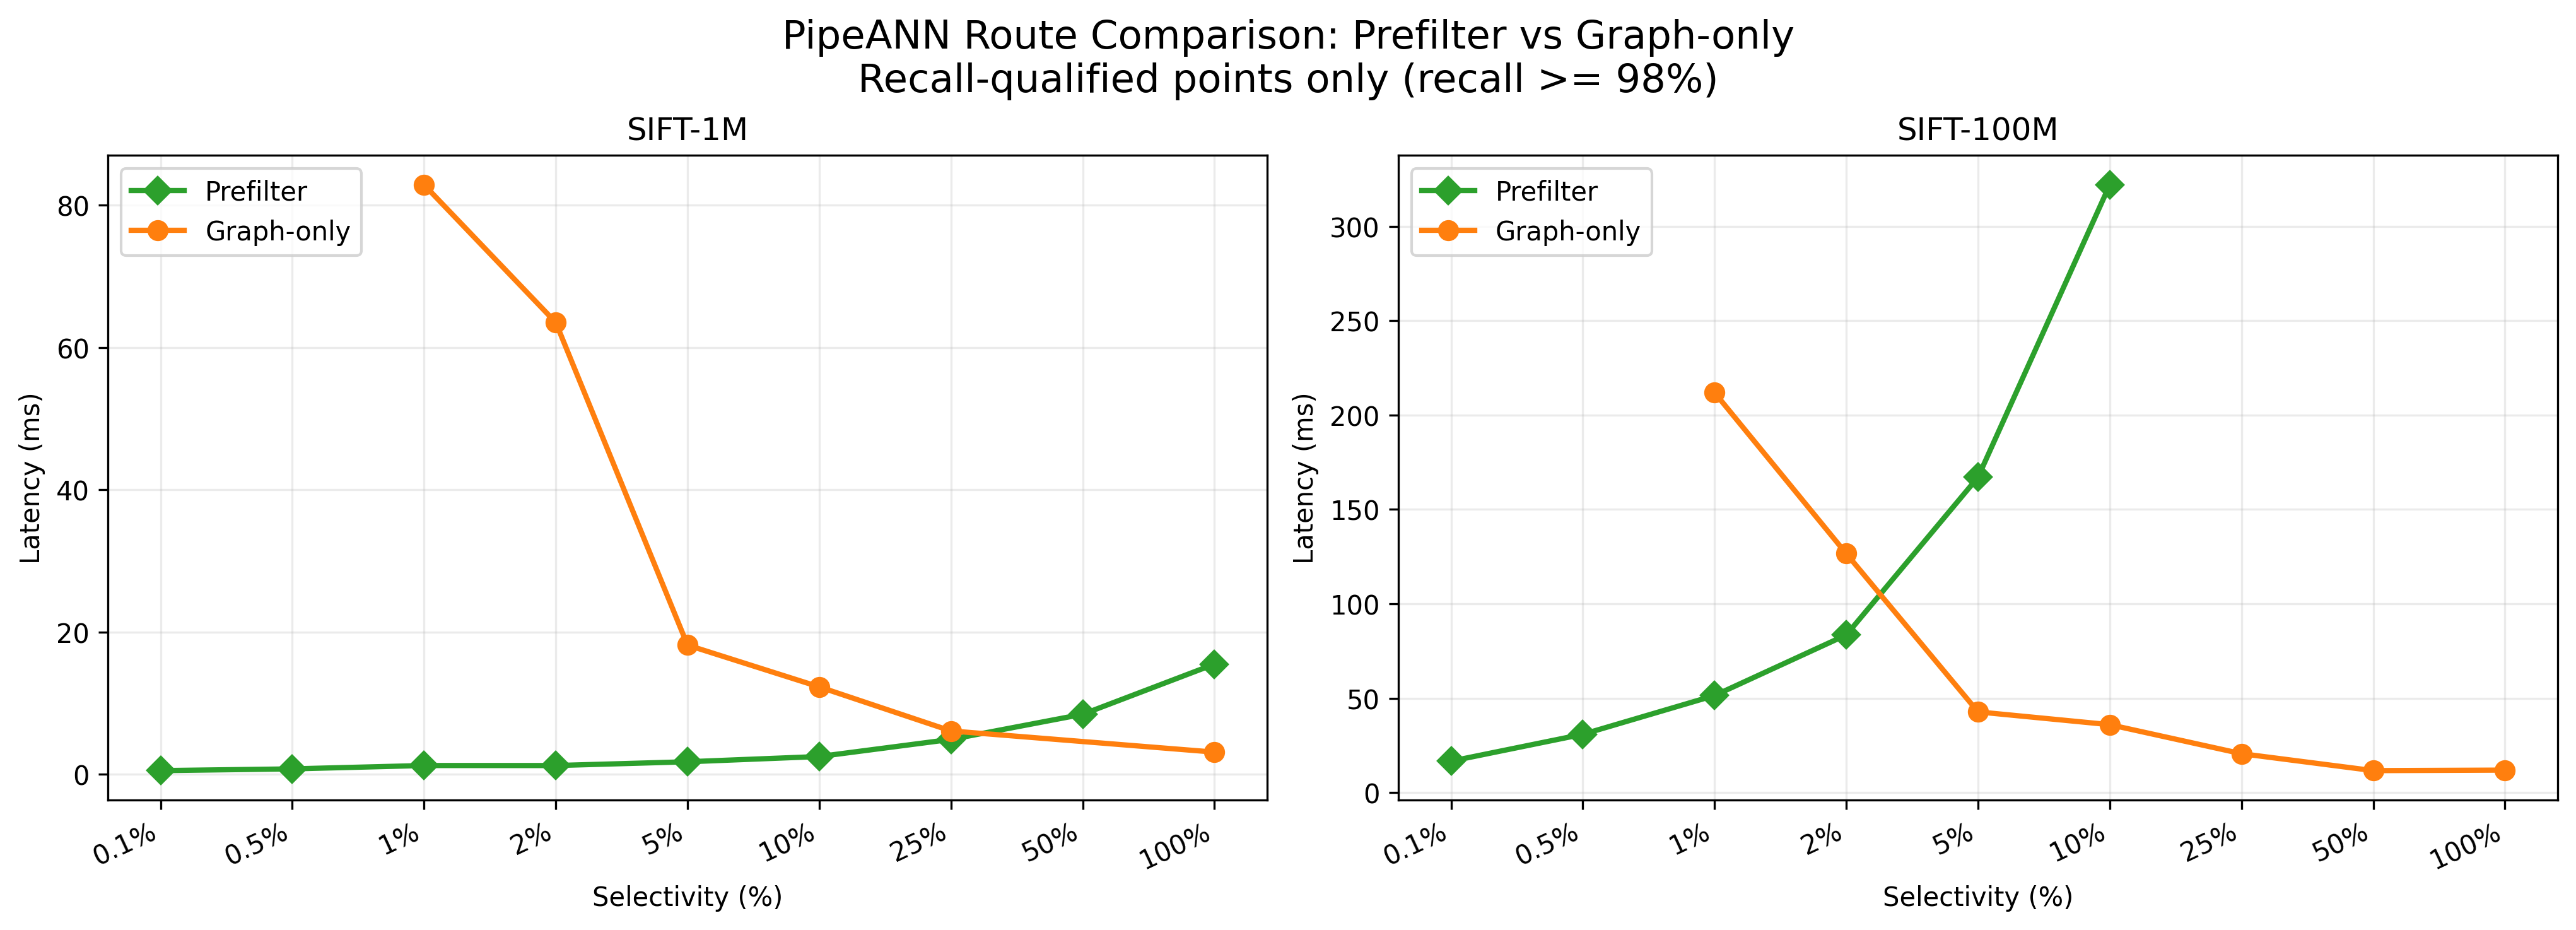
\includegraphics[width=0.93\textwidth]{figures/ppt_assets/image9.png}
\end{frame}

\begin{frame}[t]{设计点 2：位图加速过滤}
    \scriptsize
    \textbf{作用：}快速生成满足过滤条件的候选集合，避免逐向量扫描。\\[0.35em]
    \textbf{图中结论：}逐向量扫描（红线）比使用位图的方案慢 1～2 个数量级。\\[0.45em]
    \centering
    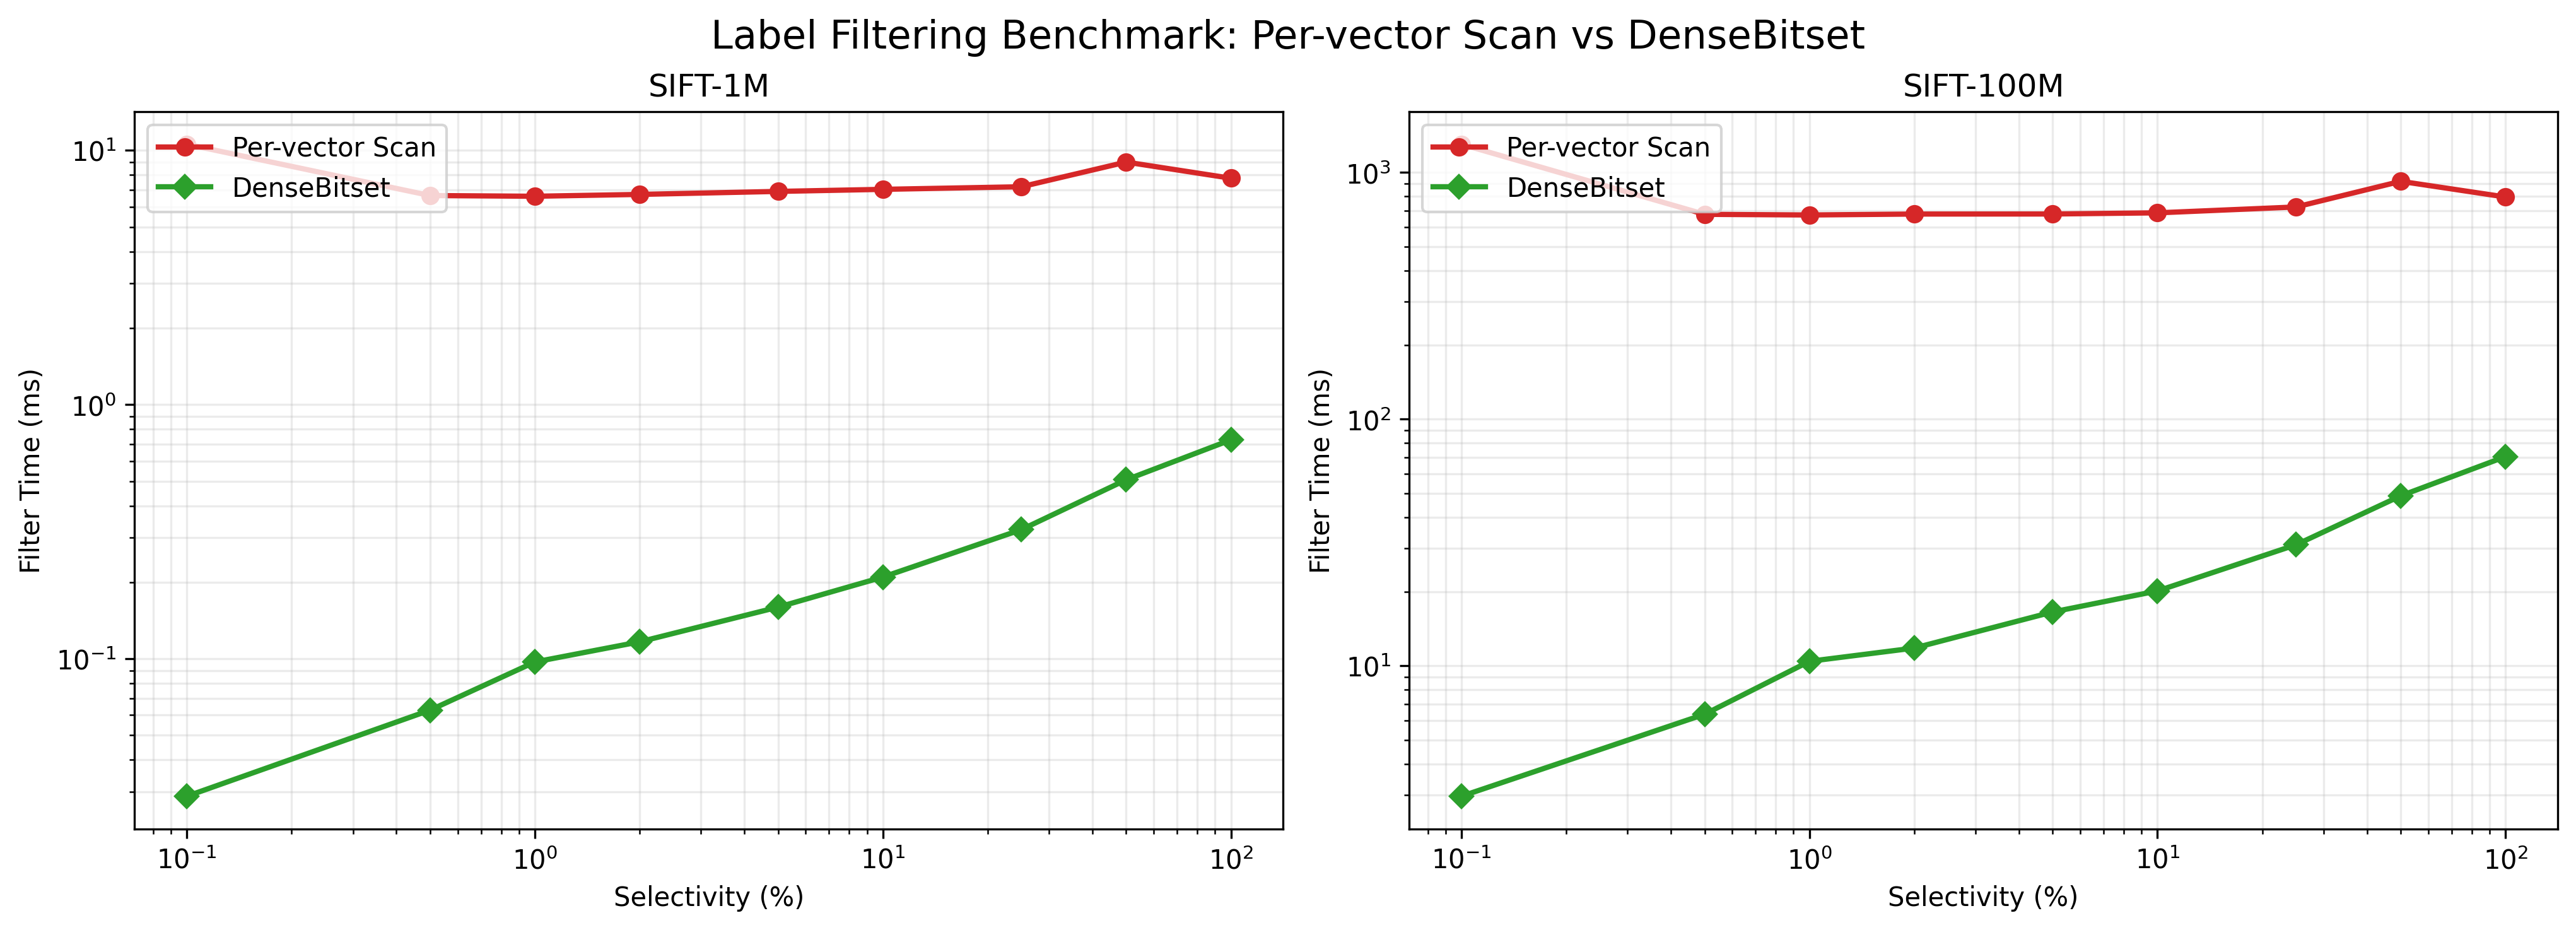
\includegraphics[width=0.95\textwidth]{figures/ppt_assets/image10.png}
\end{frame}

\begin{frame}[t]{设计点 3：PQ 候选排序与自适应重排序}
    \scriptsize
    \textbf{问题：}PQ 距离计算快，但直接返回 PQ top-$k$ 会损失召回率。\\[0.35em]
    \textbf{处理：}先用 PQ 缩小范围，再取小部分 PQ 距离最近的对象，读取原始向量做精确重排序。\\[0.35em]
    \textbf{图中结论：}取小部分对象做精确重排序即可大幅提高召回率。
    \vfill
    \centering
    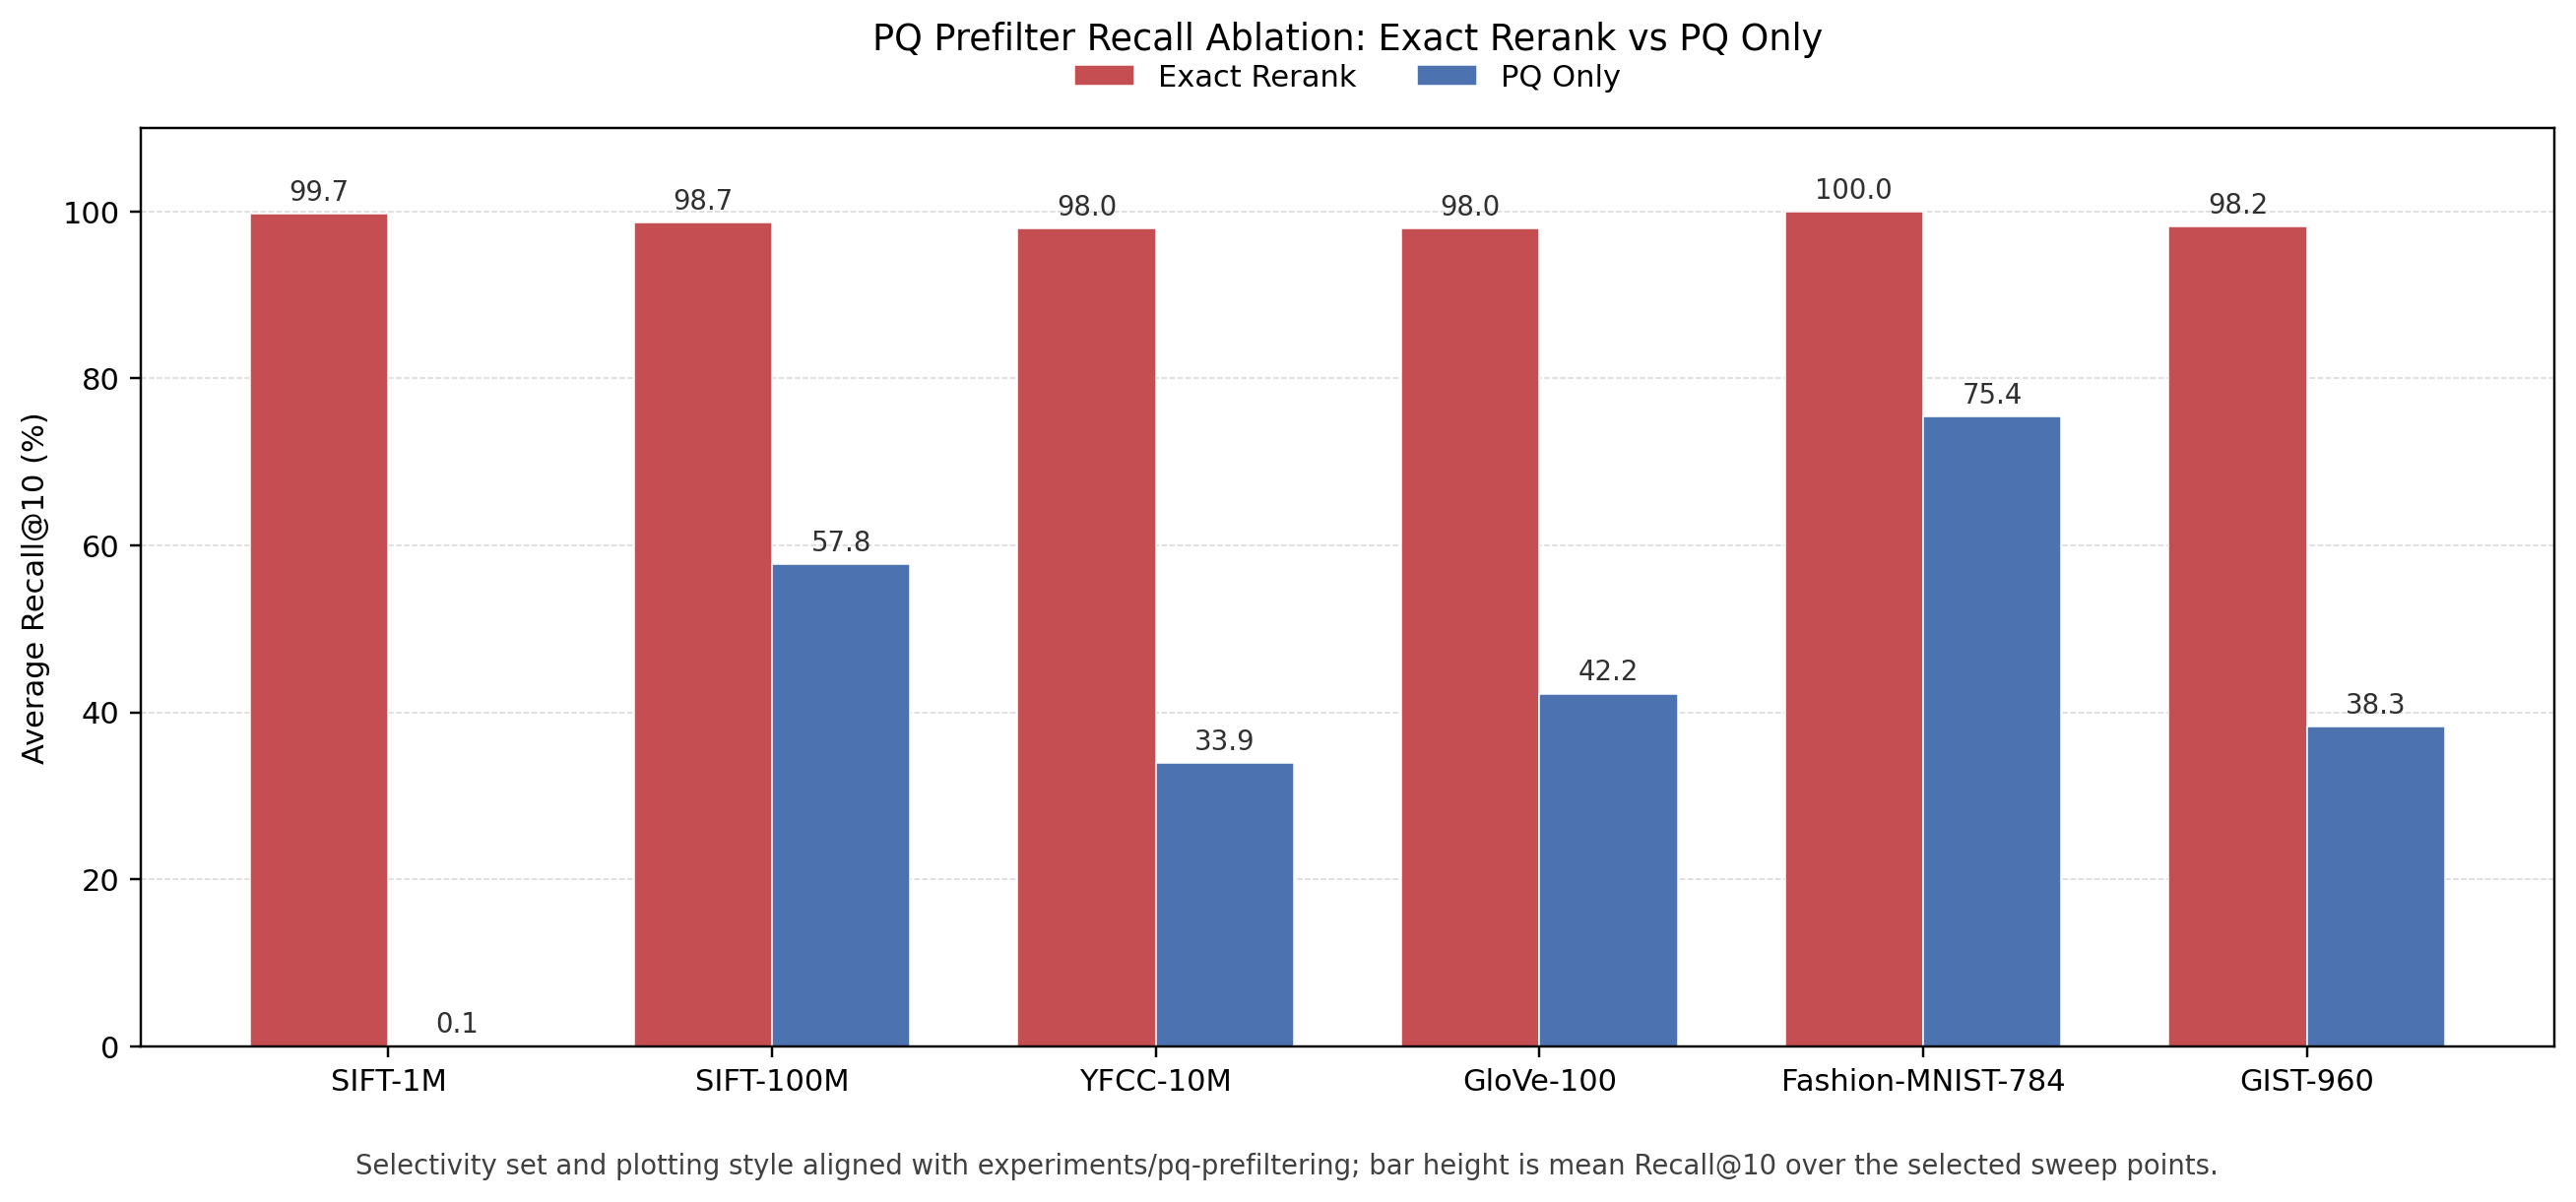
\includegraphics[width=0.74\textwidth]{figures/ppt_assets/image11.png}
\end{frame}

\begin{frame}[c]{实验设置}
    \begin{columns}[c,onlytextwidth]
        \column{0.5\textwidth}
        \scriptsize
        \begin{itemize}
            \item \textbf{实验平台}：32 核 CPU、220 GB 内存、NVMe SSD。
            \item \textbf{对比基线}：FilteredVamana (SSD)、Milvus (DISKANN)、Qdrant (HNSW)。
            \item \textbf{评价指标}：延迟、QPS、峰值内存占用。
            \item \textbf{备注}：以下实验均为在满足 Recall@10 $\geq$ 98\% 时测得的最优性能。
            \item \textbf{负载说明}：YFCC-10M 使用真实标签，其余数据集使用人工合成的标签。
        \end{itemize}

        \column{0.5\textwidth}
        \centering
        \scriptsize
        \renewcommand{\arraystretch}{1.12}
        \begin{tabular}{lcc}
            \hline
            数据集 & 规模 & 维度 \\
            \hline
            SIFT-1M & 约 100 万 & 128 \\
            GIST-960 & 约 100 万 & 960 \\
            GloVe-100 & 约 120 万 & 100 \\
            Fashion-MNIST-784 & 约 6 万 & 784 \\
            YFCC-10M & 约 1000 万 & 192 \\
            \hline
        \end{tabular}
    \end{columns}
\end{frame}

\begin{frame}[c]{实验：路径切换行为}
    \begin{columns}[c,onlytextwidth]
        \column{0.40\textwidth}
        \makebox[\linewidth][l]{%
        \begin{minipage}[c]{\linewidth}
        \small
        \begin{itemize}
            \setlength{\itemsep}{0.55em}
            \item YFCC-10M 工作负载呈长尾分布，低选择性查询占比较高。
            \item 中高选择性查询仍然存在，不能只优化单一场景。
            \item 真实负载覆盖不同候选规模，因此需要在不同路径之间自适应选择。
        \end{itemize}
        \end{minipage}}

        \column{0.60\textwidth}
        \begin{minipage}[c]{\linewidth}
        \centering
        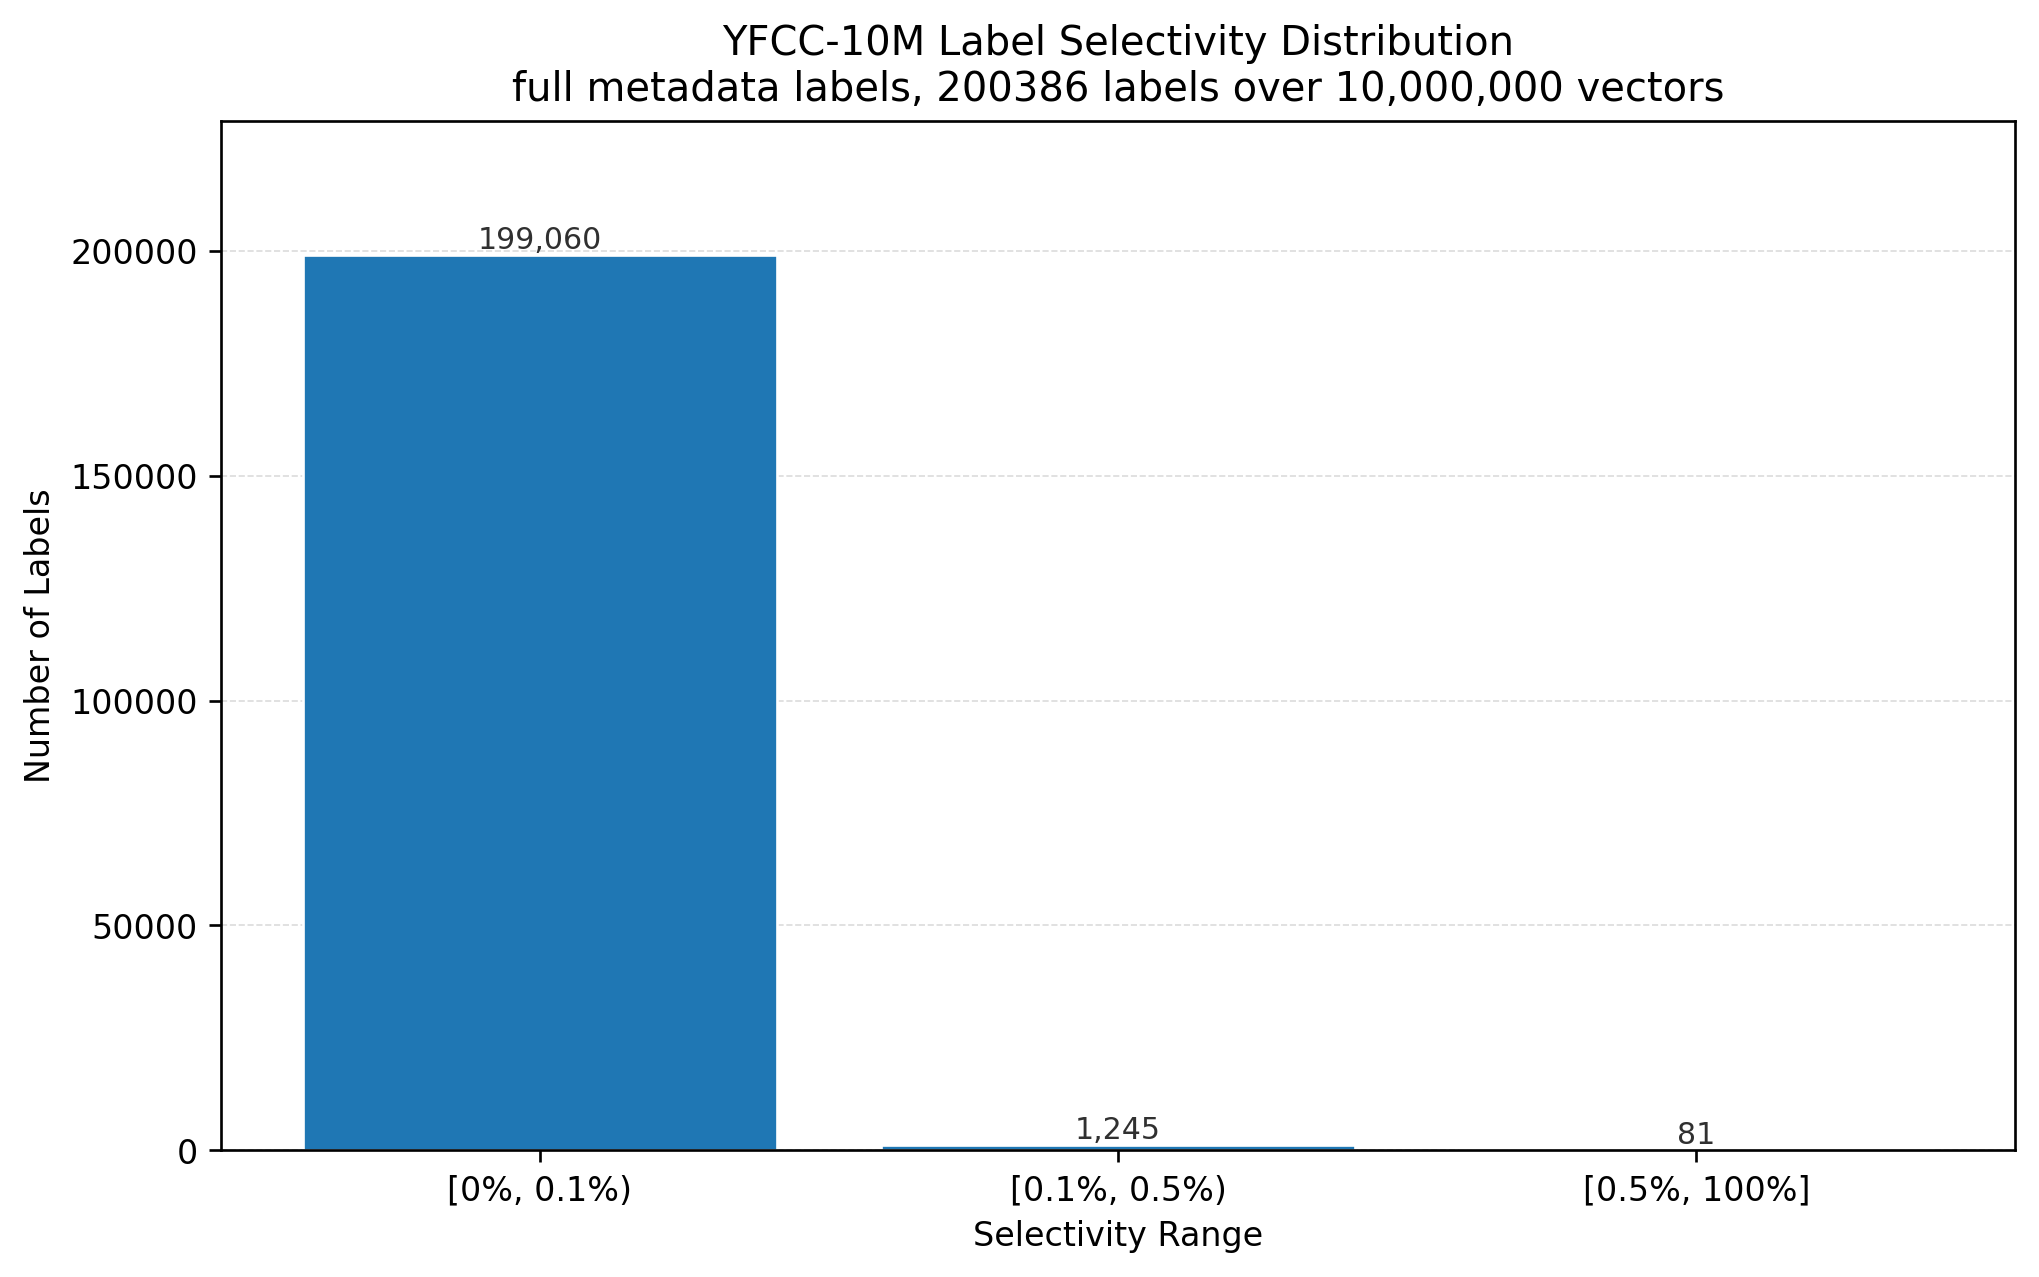
\includegraphics[width=\linewidth,height=0.62\textheight,keepaspectratio]{figures/ppt_assets/image14.png}
        \end{minipage}
    \end{columns}
\end{frame}

\begin{frame}[t]{实验：总体对比}
    \vspace*{-0.4em}
    \begin{minipage}{\textwidth}
        \footnotesize
        \begin{itemize}
            \setlength{\itemsep}{0.15em}
            \item 绿色曲线表示本文混合框架，对比延迟、QPS 与峰值内存占用。
            \item 在保持性能接近的同时，可以降低 1～2 个数量级的内存占用。
        \end{itemize}
    \end{minipage}
    \vspace*{-0.5em}
    \centering
    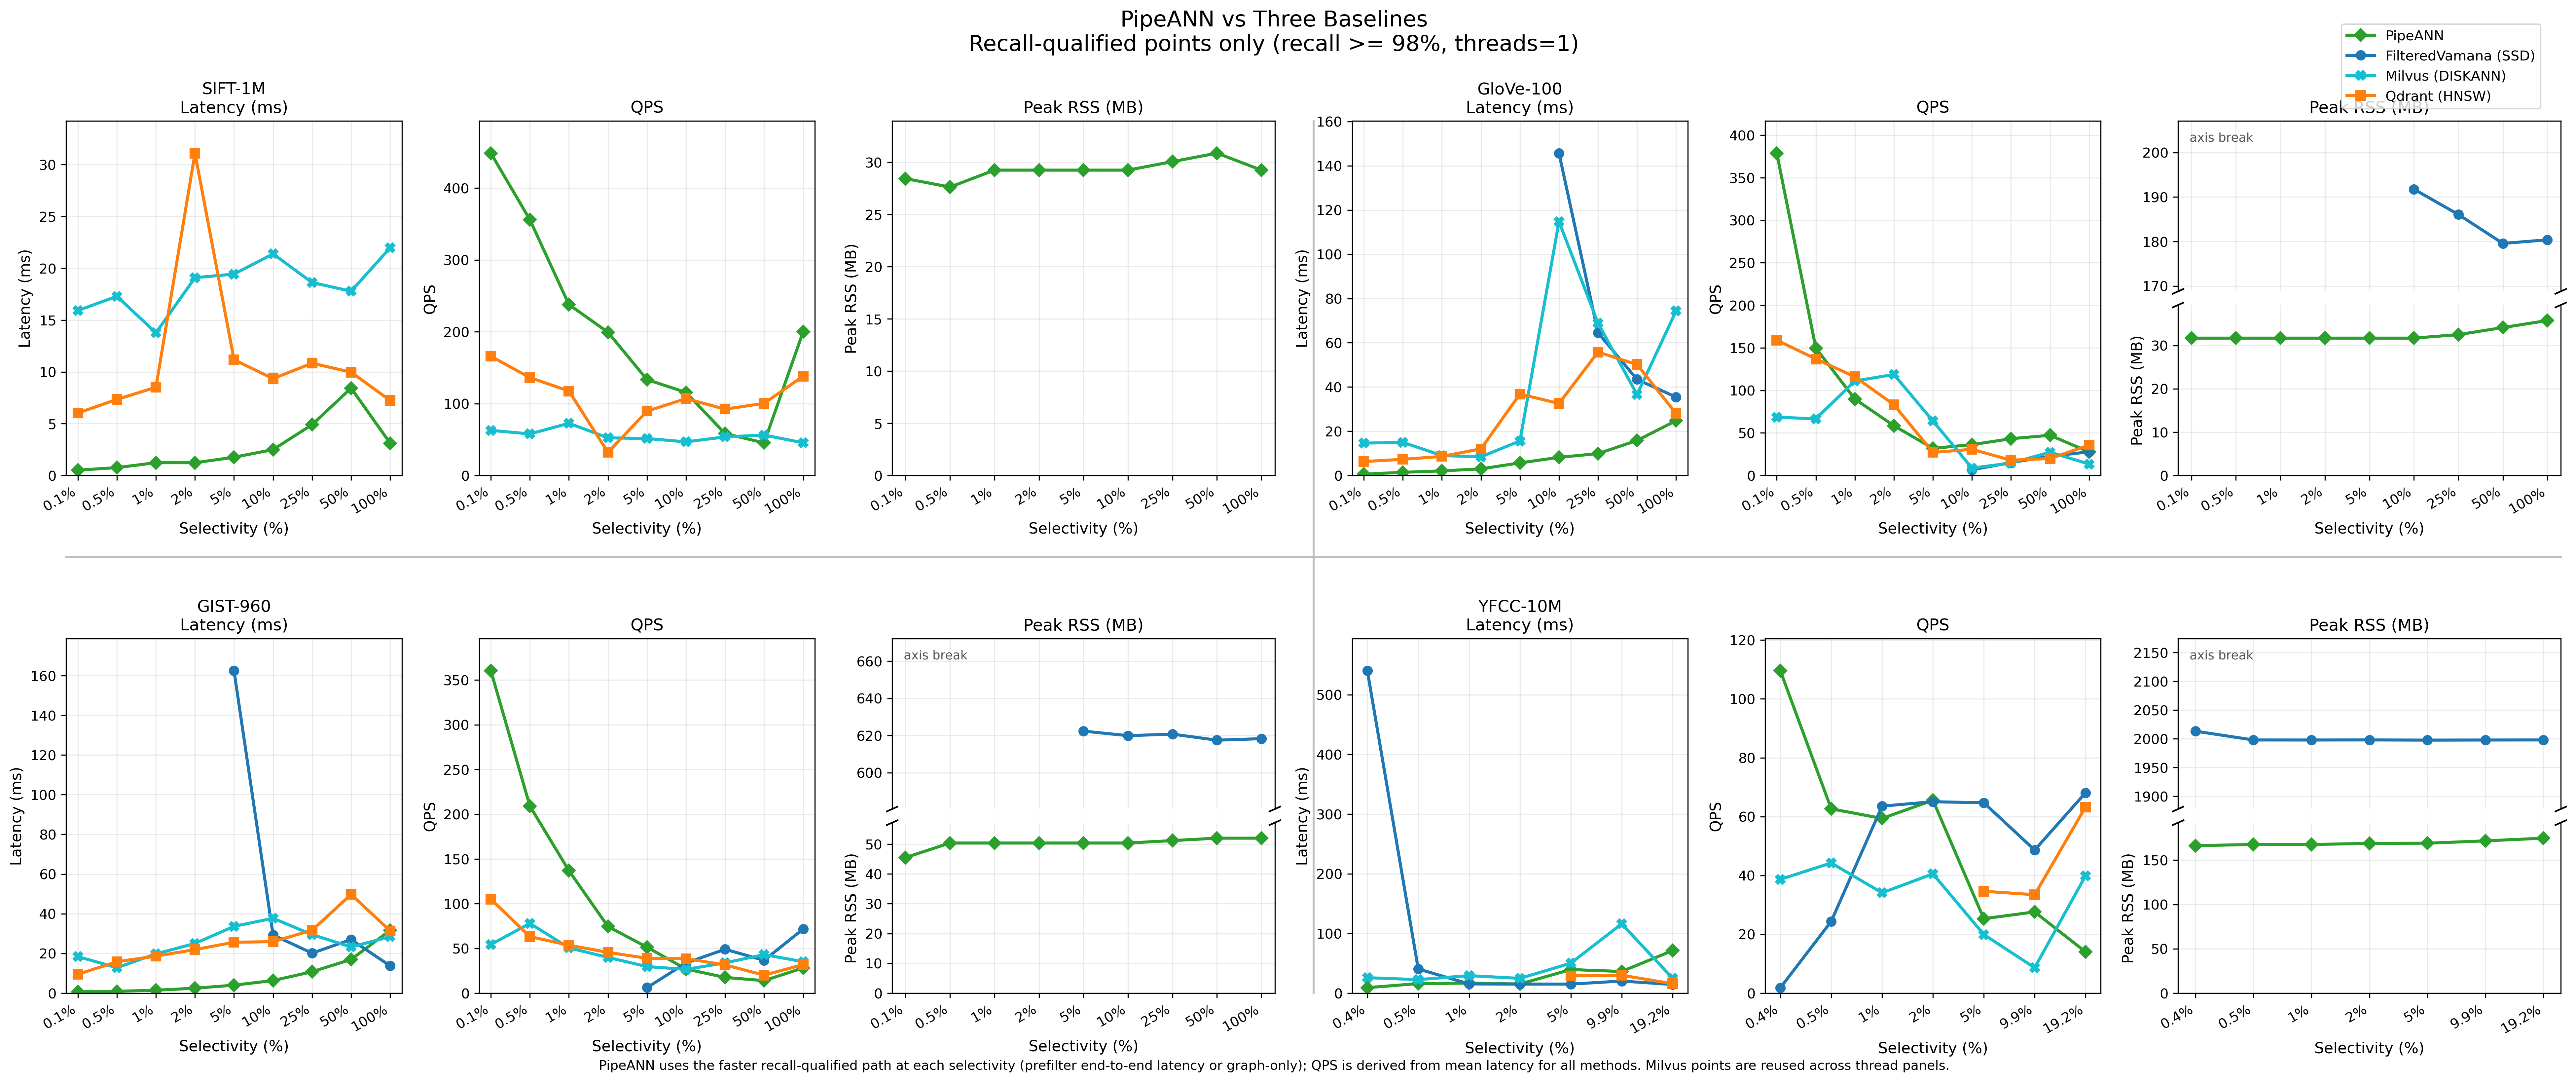
\includegraphics[width=\textwidth,height=0.78\textheight,keepaspectratio]{figures/ppt_assets/compare_4sets_2x6.png}
\end{frame}

\begin{frame}[c]{实验：多线程扩展性}
    \begin{columns}[c,onlytextwidth]
        \column{0.32\textwidth}
        \makebox[\linewidth][l]{%
        \hspace*{-0.7em}%
        \begin{minipage}[c]{\dimexpr\linewidth+0.7em\relax}
        \scriptsize
        \begin{itemize}
            \item 测试 1、2、4、8 线程下的吞吐变化。
            \item 多数数据集上 QPS 随线程数提升，说明框架具备并行扩展能力。
            \item 高选择性下增加线程数的性能提升较小，说明瓶颈逐渐转向 SSD IO。
        \end{itemize}
        \end{minipage}}

        \column{0.68\textwidth}
        \hspace*{0.7em}%
        \begin{minipage}[c]{\dimexpr\linewidth-0.7em\relax}
        \centering
        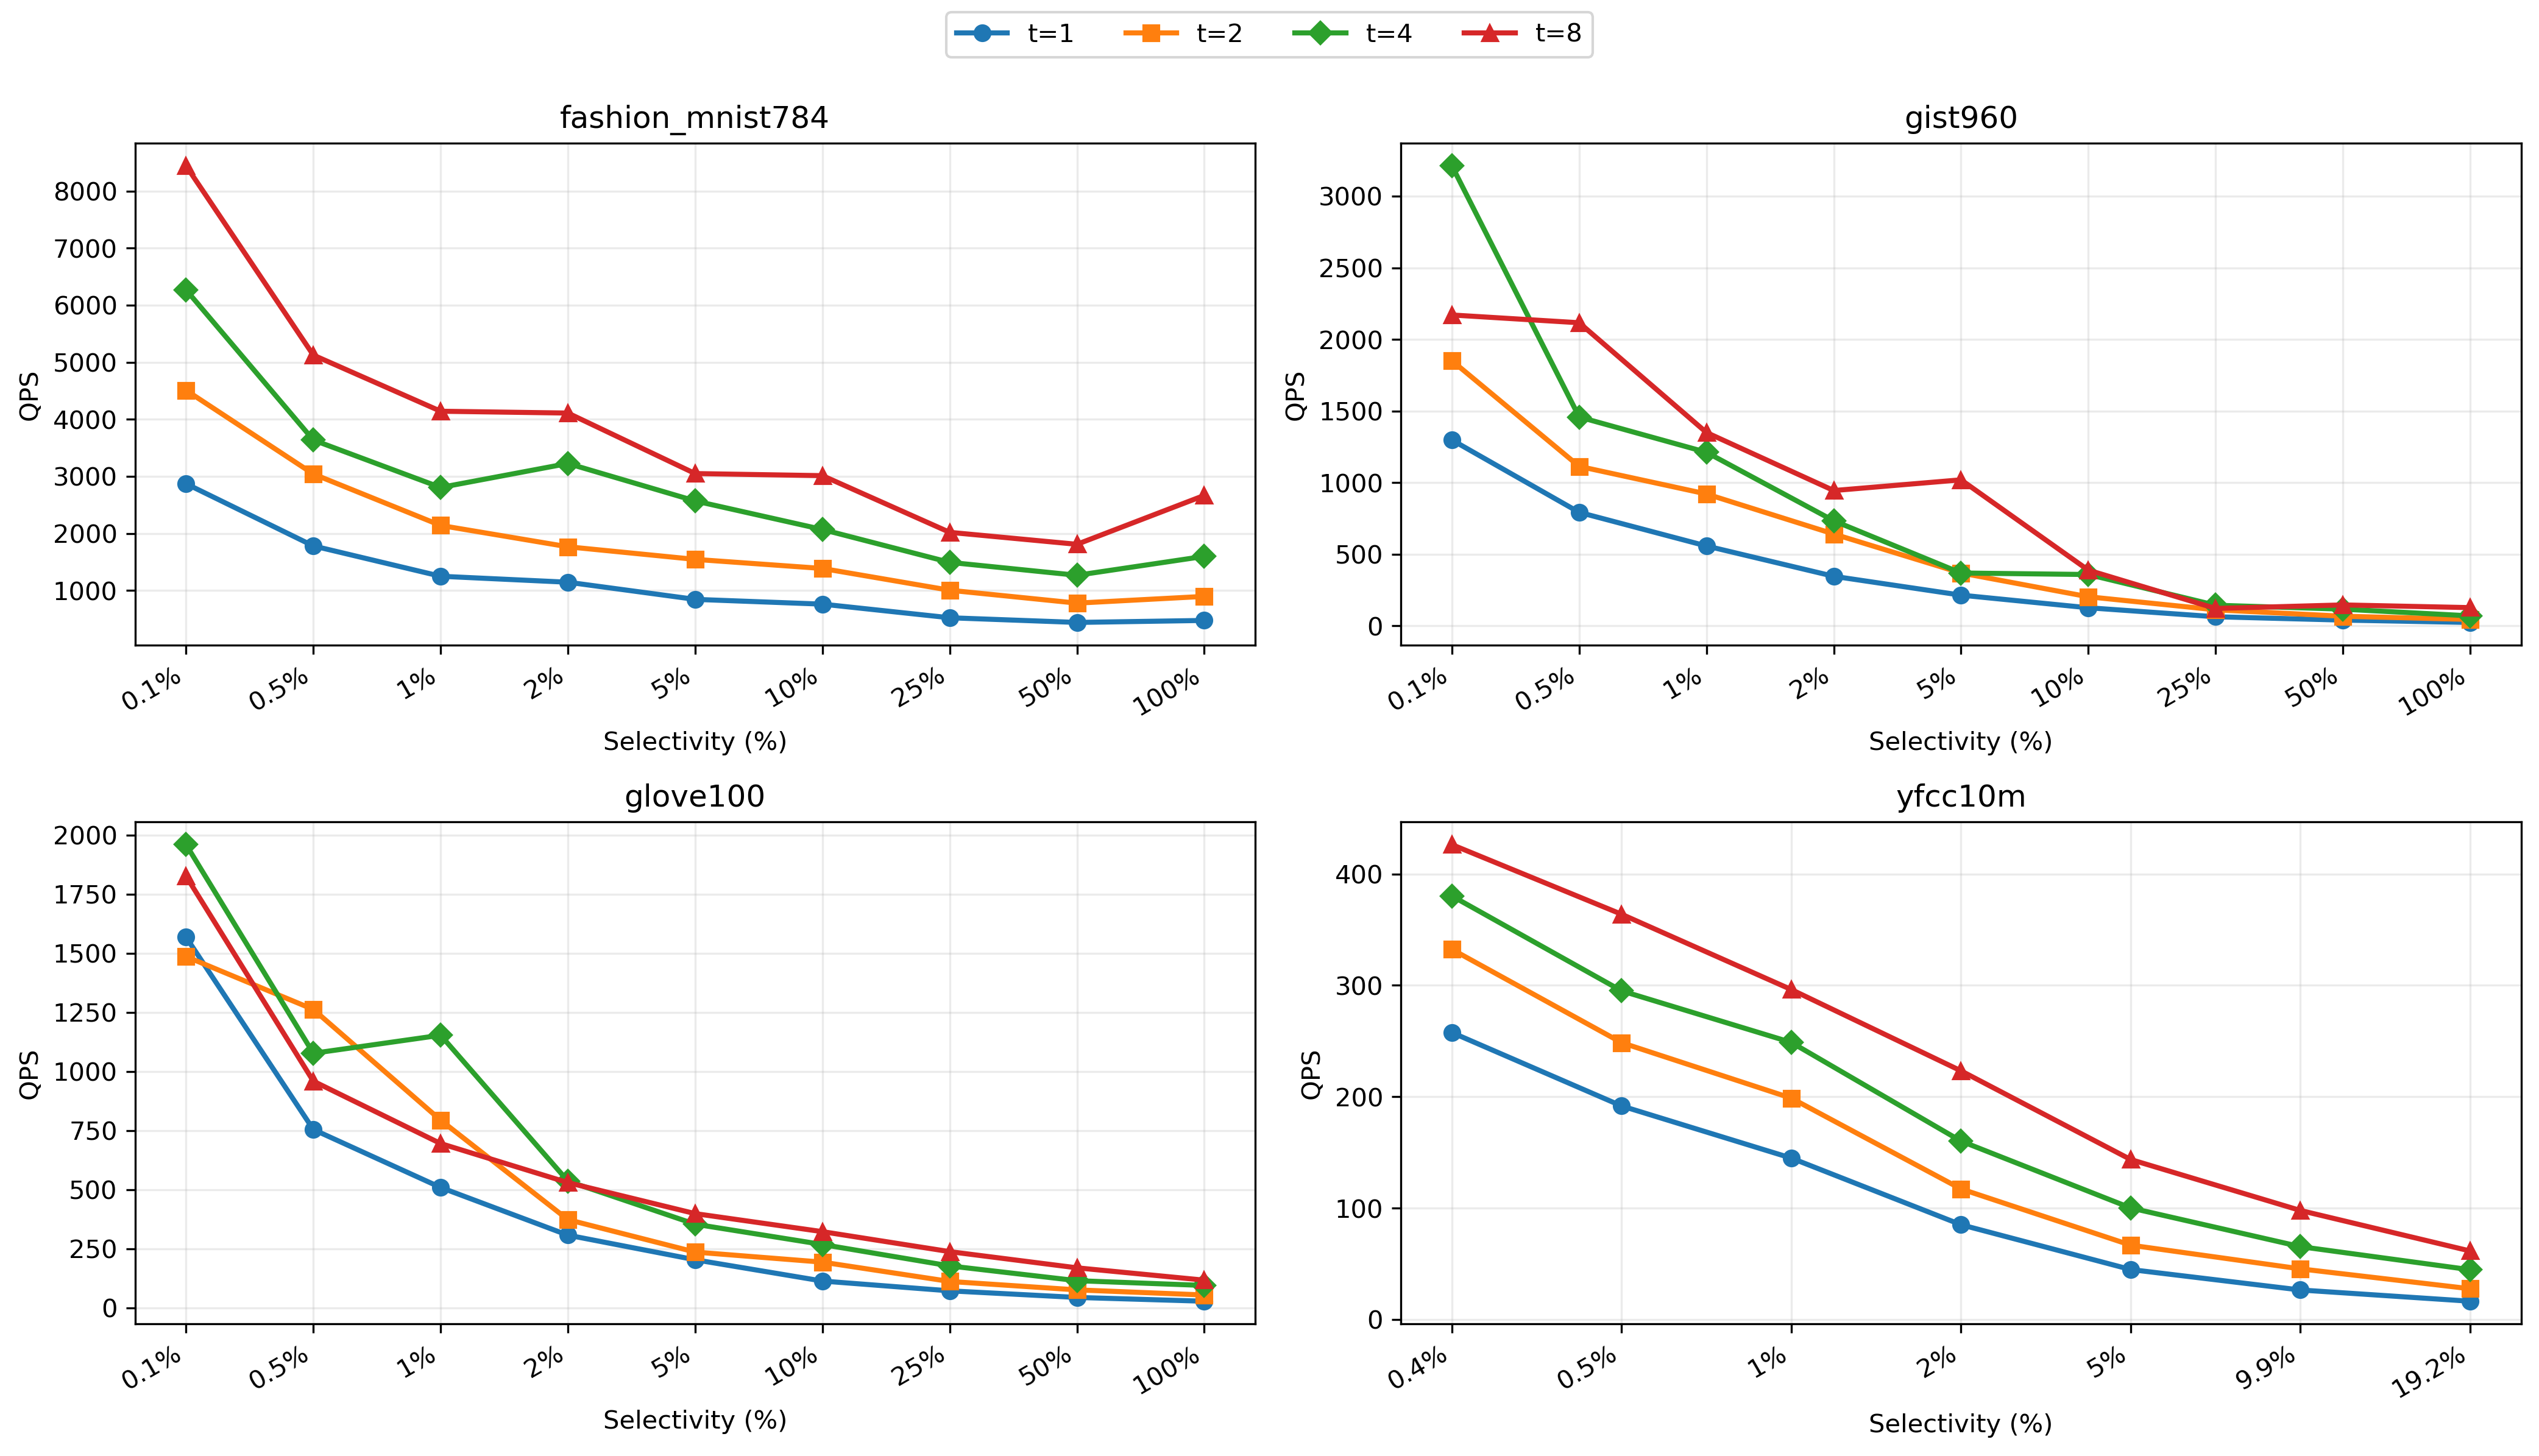
\includegraphics[width=\linewidth,height=0.78\textheight,keepaspectratio]{figures/ppt_assets/qps_4sets.png}
        \end{minipage}
    \end{columns}
\end{frame}

\thanksforlistening{请各位老师批评指正}

\end{document}
